\chapter{Einleitung}
Hören die meisten Personen die Begriffe \enquote{Künstliche Intelligenz}
und \enquote{Maschinelles Lernen} stellen sie sich Roboter vor:
treue Diener, die all deine Aufgaben übernehmen oder eine tödliche Arme
von superintelligenten Cyborgs im Kampf gegen die Menschheit.
Künstliche Intelligenz (kurz KI) ist jedoch schon lange nicht mehr nur eine futuristische
Fantasie und Teil von Science-Fiction-Filmen; es wird bereits großflächig
eingesetzt und findet Verwendung in einer Vielzahl von Anwendungen aus Bereichen
in nahe zu allen Teilen der Wirtschaft. Andrew Ng,
welcher unteranderem durch seine beliebten Onlinekurse zum Thema
Maschinellen Lernen (ML) und Deep Learning (DL)
bekannt ist,
\footnote{\url{https://www.coursera.org/instructor/andrewng}}
vergleicht KI mit der neuen Elektrizität.
\begin{aquote}{Andrew Ng \parencite{online:ai-andrew-ng}}
  \enquote{\textit{Just as electricity transformed almost everything 100 years ago,
      today I actually have a hard time thinking
      of an industry that I don’t think AI will
      transform in the next several years}}
\end{aquote}
Die Anwendung, mit der Maschinelles Lernen erstmalig öffentliche Aufmerksamkeit
erlangte und und noch immer das tägliche Leben vieler Menschen beeinflusst,
stammt aus den 90er-Jahren:
Die Rede ist von dem E-Mail-Spamfilter \parencite[1]{book:hands-on-ml}.
Es handelt sich um eine scheinbar einfache Aufgabe, welche
mit traditioneller Programmierung aber dennoch nur schwer gelöst werden kann.
Ein klassisches Programm besteht aus vielen statischen Regeln,
im Fall des Spamfilters können diese dazu dienen, auffällige Schlüsselwörter und
Satzteile zu erkennen (wie \enquote{Kreditkarte}, \enquote{konstenlos}, \enquote{kaufen} oder
andere Merkmale).
Ein statisches Programm ist nicht gut dafür geeignet, ein dynamisches Problem
zu beschreiben. Die Absender der Spamnachrichten könnten erkennen, welche E-Mails blockiert werden
und diese leicht abändern. Arbeiten sie so durchgehend um das Problem herum,
müssen immer wieder neue Regeln im Programm aufgenommen werden. Ein Spamfilter hingen,
welcher auf Maschinellen Lernen basiert, kann diese Regeln
selbstständig erkennen und automatisch anpassen wenn es eine Veränderung erkennt.
Der Algorithmus durchläuft eine Trainingsphase und verwendet dabei
Beispiel E-Mails (z.\,B. diese, die vom Benutzer markiert wurden)
und kann so lernen Spamnachrichten zu unterscheiden.
Diese Trainingsdaten werden als Trainingsdatensatz (engl. \textit{train set})
bezeichnet.
Es folgt ein Programm, welches weitaus kürzer,
einfacher zu verwalten und wahrscheinlich auch präziser ist.

\section{Was ist Maschinelles Lernen?}
Maschinelles Lernen ist die Wissenschaft (und Kunst) der Programmierung,
die es dem Computer ermöglicht, von Daten zu lernen. Arthur Samuel und Tom Mitchell
haben im Jahr 1959 und 1997 eine allgemeine und formale Definition gegeben \parencite[2]{book:hands-on-ml}:
\begin{aquote}{Arthur Samuel, 1959}
  \enquote{\textit{Machine Learning is the field of study that gives computers
      the abilty to learn without being explicitly programmed.}}
\end{aquote}
\begin{aquote}{Tom Mitchell, 1997}
  \enquote{\textit{A computer program is said to learn from experience
      $E$ with respect to some task \,$T$ and some performance measure $P$,
      if its performance on $T$, as measured by $P$, improves with experience $E$.}}
\end{aquote}
Betrachten wir erneut das Beispiel des Spamfilters, dann ist die Aufgabe $T$
das Markieren von Spam, die Erfahrung
$E$ sind die Trainingsdaten ist und der Bewertungsmaßstab $P$ bleibt zu definieren.
Es könnte zum Beispiel der Anteil der als richtig markierten E-Mails verwendet
werden. Dieser Maßstab heißt Genauigkeit und wird
häufig verwendet wenn es darum geht eine Klassifizierungsaufgabe zu bewerten.

\section{Die unterschiedlichen Lernmethoden}
\label{sec:lernmethoden}
Maschinelles Lernen kann genutzt werden, um eine Vielzahl von Problemen zu lösen.
Dies macht es zu einem mächtigen Werkzeug, aber auch eines, in dem es schwierig sein
kann, den Überblick zu behalten.
Da es viele verschiedene Systeme, Architekturen und Lösungsansätze gibt, ist es sinnvoll,
diese in grobe Kategorien zu unterteilen.
Ein System kann unterschieden werden, basierend auf den folgenden
Kriterien \parencite[7]{book:hands-on-ml}:
\begin{itemize}
  \item Trainiert das System mit oder ohne menschlicher Betreuung, dann ist
        die Rede von überwachten und unüberwachten Lernen.
  \item Kann das System inkrementell mit einer Teilmenge der Trainingsdaten
        lernen oder verwendet es die gesamten Daten. Dieser Unterschied
        nennt sich Online- vs. Batch-Learning.
  \item Funktioniert das System indem es lediglich neue Daten mit
        den alten vergleicht oder kann es Muster erkennen, um beispielsweise
        einen Datensatz in Klassen zu unterteilen.
        Diese Lernmethoden nennen sich instanzbasiertes und modellbasiertes Lernen.
\end{itemize}
Keine der eben beschriebenen Kriterien schließen sich aus.
In einem echten System kann es sinnvoll sein, die verschiedenen
Eigenschaften zu kombinieren, um das gewünschte Ergebnis
zu erzielen. Der zuvor beschriebene E-Mail-Spamfilter
ist ein klassisches überwachtes und instanzbasiertes Lernsystem.
Es ist überwacht, da der Typ der E-Mail (z.\,B. durch Benutzereingabe)
bekannt ist und instanzbasiert da
der Algorithmus neue E-Mails mit alten vergleicht und das
Ergebnis so wählt, worin die größte Ähnlichkeit besteht.
Die Ergebnisse beim überwachten Lernen können wie im Falle des
Spamfilters vom Benutzer stammen oder durch Naturgesetzte und Expertenwissen
gegeben sein. Diese Daten werden als Label bezeichnet.
Wir können nun die einzelnen Lernmethoden etwas genauer untersuchen.

\paragraph{Klassifizierung versus Regression}
Das bisherige Spamfilter Beispiel ist ein typisches
Klassifizierungsproblem. Zu einer Menge von eine Eingabewerten
(auch genannt Features) soll die Wahrscheinlichkeit bestimmt werden,
dass diese Feature zu einer bestimmten Klasse gehören.
Was ist aber wenn keine Wahrscheinlichkeiten
prognostiziert werden sollen, sondern numerische Werte wie
der Preis eines Autos? Dieses Problem nennt sich Regression.
Ein Beispiel wird zeigen, wie das Prinzip funktioniert.
Es soll ein einfaches Modell trainiert werden welches eine lineare
Funktion modelliert. Als ersten Schritt müssen die Trainingsdaten generiert werden.
Der folgende Python Code zeigt diesen Vorgang mithilfe von NumPy:
\begin{lstlisting}
import numpy as np
rng = np.random.default_rng(42)
x = 6 * rng.random((100, 1))
y = 5 + 3 * x
\end{lstlisting}
NumPy ist eine Python Bibliothek, die effiziente Berechnungen mit
multidimensionalen Daten ermöglicht (z.\,B. der Vektor- und Matrixmultiplikation).
\footnote{\url{https://numpy.org/doc/stable/user/whatisnumpy.html\#what-is-numpy}}
Operationen in NumPy werden immer elementweise durchgeführt. Der folgende Programmausschnitt
zeigt dieses Verhalten:
\begin{lstlisting}
>>> a = np.array([1, 2, 3])
>>> a
°array([1, 2, 3])°
>>> a * 3
°array([3, 6, 9])°
\end{lstlisting}
CPUs und GPUs sind sehr gut darin, diese Art der Berechnungen durchzuführen,
was NumPy sehr viel schneller macht als die Verwendung einer expliziten Schleife.
Die Technik, nicht mehr nur mit skalaren Werten zu rechnen,
nennt sich Vektorisierung und kann
die Laufzeit eines rechenintensiven Algorithmus
(wie sie in der KI zum Einsatz kommen) drastisch verringern.
\begin{aquote}{\parencite{online:vectorization}}
  \enquote{\textit{Vectorization is the process of converting an algorithm
      from operating on a single value at a time to
      operating on a set of values (vector) at one time}}
\end{aquote}
Wir können nun die zuvor generierten Daten visualisieren und verwenden hierfür
eine weitere Python Bibliothek mit dem Namen Matplotlib:
\footnote{\url{https://matplotlib.org/stable/index.html}}
\begin{lstlisting}
import matplotlib.pyplot as plt
plt.plot(x, y, "b.")
plt.xlabel("$x_1$")
plt.ylabel(r"$5 + 3x$")
plt.axis([0, 6, 5, 25])
plt.show()
\end{lstlisting}
Die hieraus resultierende Grafik ist in \autoref{plot:linear-data} zu sehen.

\begin{figure}[!h]
  \centering
  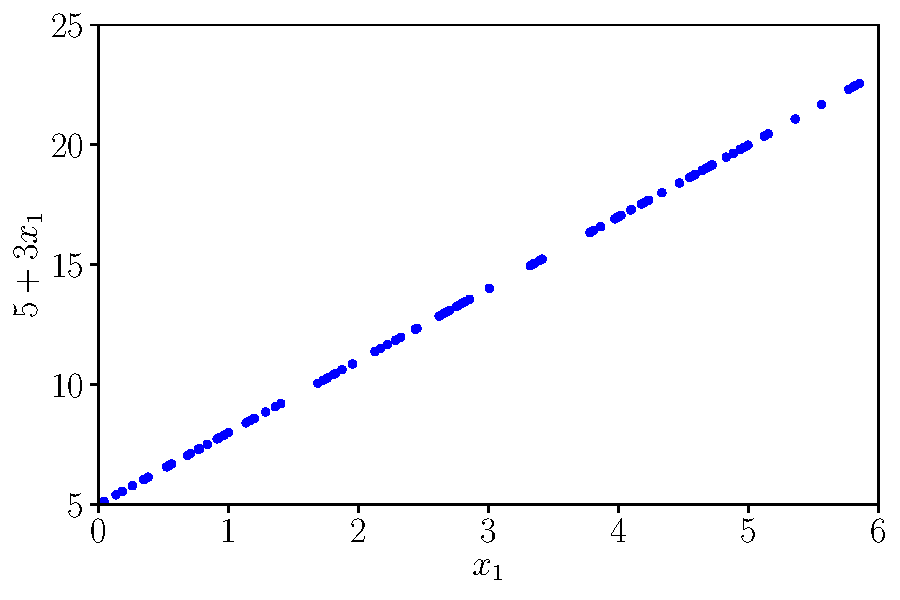
\includegraphics[width=0.55\textwidth]{einleitung/linear-data.pdf}
  \caption{Die generierte Daten}
  \label{plot:linear-data}
\end{figure}

\noindent
Die Daten sehen sehr gerade aus, damit das Problem nicht zu einfach ist
addieren auf Seiten der $y$ Werte zufälliges Rauschen.
\begin{lstlisting}
y += 3 * rng.standard_normal((100, 1))
\end{lstlisting}
Dies sollte das Problem ein wenig realistischer gestallten.
Die so modifizierten Daten sind in \autoref{plot:linear-data-noise} zu sehen.
\begin{figure}[!h]
  \centering
  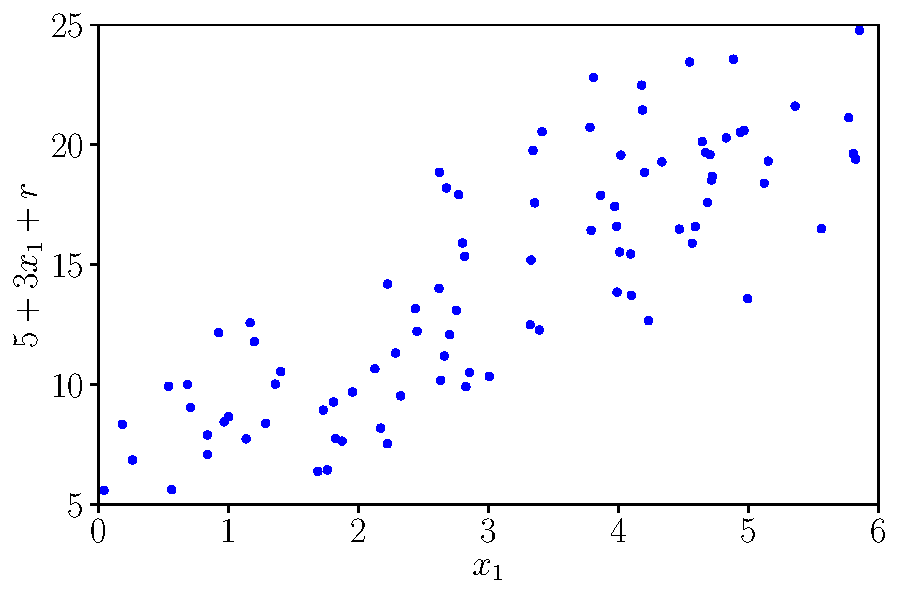
\includegraphics[width=0.55\textwidth]{einleitung/linear-data-noise.pdf}
  \caption{Die generierte Daten plus zufälliges Rauschen}
  \label{plot:linear-data-noise}
\end{figure}
Das Regressionsproblem besitzt eine Eingabe $x_1$ und eine Ausgabe $y$.
Ein echtes Problem besteht in der Regel aus mehreren Eingaben und manchmal
aus mehreren Ausgaben. Mehrdimensionale Daten lassen sich allerdings nur schwierig
visualisieren. Ziel des Modells ist es nun eine Gerade zu finden, welche die
Daten möglichst gut beschreibt. Die Geradengleichung hat die folgende Form:
\begin{align}
  \text{1 Feature}\qquad    & \yhat = \theta_0 + \theta_1 \cdot x_1   \\
  \text{$n$ Features}\qquad & \yhat = \theta_0 + \theta_1 \cdot x_1 +
  \theta_2 \cdot x_2 + \ldots + \theta_n \cdot x_n
\end{align}
Die griechischen Buchstaben Theta $\theta_i$ beschreiben die lernbaren Parameter und
der Funktionswert $\yhat$ (gesprochen \enquote{y-Hut}) beschreibt die Prognose.
Das Training kann in Python mit nur wenigen Zeilen Code durchgeführt werden:
\begin{lstlisting}
from sklearn.linear_model import LinearRegression
lin_reg = LinearRegression()
lin_reg.fit(x, y)
\end{lstlisting}
Wir verwenden das \lstinline{LinearRegression} Modell von Scikit-Learn
\footnote{\url{https://scikit-learn.org/stable/}} und rufen die \lstinline{fit}
Methode zusammen mit den Trainingsdaten und Labels auf, um das Modell zu trainieren.
Die trainierten Parameter befinden sich in den Attributen \lstinline{intercept_}
und \lstinline{coef_}:
\begin{lstlisting}
>>> lin_reg.intercept_, lin_reg.coef_
°(array([4.84609918]), array([[3.03831479]]))°
\end{lstlisting}
Nicht schlecht: Das Modell vermutet $\yhat = 4.85 + 3.04x_1$, wobei die ursprünglich
Funktion $y = 5 + 3x_1 + r$ war. Die genauen Werte konnten aufgrund des Rauschens
nicht wiedergewonnen werden. Die Regressionsgerade ist
in \autoref{plot:linear-data-prediction} zu sehen.
\begin{figure}[!h]
  \centering
  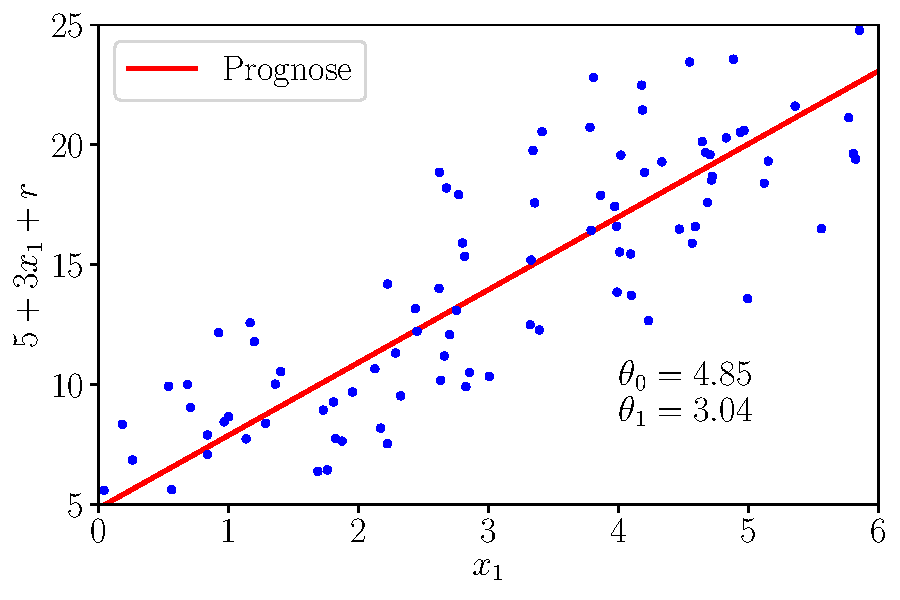
\includegraphics[width=0.55\textwidth]{einleitung/linear-data-prediction.pdf}
  \caption{Regressionsgerade}
  \label{plot:linear-data-prediction}
\end{figure}

\paragraph{Batch- und Online-Learning}
Ein weiterer Punkt, anhand dessen ein KI-System unterschieden
werden kann, ist die Methode, wie es Daten verarbeitet \parencite[15]{book:hands-on-ml}.
Dieser Unterschied nennt sich Batch- und Online-Learning.
Beim Batch-Learning werden Daten stapelweise verarbeitet.
Das Modell bzw. die Parameter werden erst dann angepasst,
nachdem der gesamte Stapel (Batch) das Training durchlaufen hat.
Dies braucht in der Regel viel Zeit und Speicherkapazität, weshalb
es typischerweise offline durchgeführt wird.
Nachdem ein System veröffentlicht wurde, wendet es, dass an, was es gelernt hat,
kann aber keine neuen Schlüsse mehr ziehen.
Soll das System auf neue Daten reagieren, muss ein neues Modell trainiert werden.
Das Online-Learning funktioniert anders.
Im Training werden die Daten nicht stapelweise verarbeitet,
sondern einzeln nacheinander.
Dies spart Zeit und Platz und kann hilfreich sein, wenn es darum geht,
mit sehr großen Datensätzen zu trainieren, die nicht alle gleichzeitig
in den Speicher passen würden.
Ein weiterer Vorteil ist der, dass neue Daten spontan auf dem Weg
verarbeitet werden können. Online-Learning eignet sich also gut,
um kontinuierliche Daten zu analysieren (z.\,B. Aktienkurse).

\section{Beschreibung des Problems}
In dieser Bachelorarbeit geht es um Maschinelles Lernen auf mobilen Geräten.
Zu Beginn der Arbeit stellte sich der Autor die Frage:
\enquote{Wie kann ein System entwickelt werden, mit dem verschiedene KI-Modelle
  verwaltet werden können, welches modular und einfach erweiterbar ist
  und über gemeinsame Schnittstellen im Netz kommuniziert?}
Das System soll gut zusammen mit der Idee des Internets der Dinge
(engl. Internet of Things, IoT) integriert werden können.
Die Modularität ist deshalb wichtig, da auch IoT aus vielen vernetzten
Einzelelementen besteht.
Der restliche Teil dieser Arbeit wird sich mit einer
speziellen Form von KI-Systemen beschäftigen: diese sind künstliche
neuronale Netze. Die Natur hat bereits eine unzählige Menge von Erfindungen
inspiriert, es liegt daher nahe, die Funktionsweise des Gehirns zu
untersuchen, um ein intelligentes System zu entwickeln.
Der Prozess, ein neuronales Netz zu trainieren, nennt sich Deep Learning (DL).
DL ist keine neue Idee:
Der Neurophysiologie Warren McCulloch und der Mathematiker Walter Pitts
haben das Prinzip im Jahr 1943 erstmalig öffentlich eingeführt
\parencite[280]{book:hands-on-ml}. Der frühe Erfolg von neuralen
Netzen brachte Enthusiasmus und große Erwartungen,
doch als sich in den 70er-Jahren herausstellte, dass diese Erwartungen nicht erfüllt
werden können, verlangsamte sich die Forschung und die Fördermittel
wurden weniger \parencite[280]{book:hands-on-ml}.
Es ist nur kürzlich, dass neuronale Netze einen neuen Aufschwung erleben
und dies wahrscheinlich nicht mehr eine Wiederholung der Vergangenheit ist.
Die folgenden Punkte begründen diese Vermutung \parencite[280]{book:hands-on-ml}:
\begin{itemize}
  \item Durch die immer stärker digitalisierte Welt
        entstehen sehr große Mengen an Daten.
        Die Forschung und Praxis hat gezeigt, dass tiefe neuronale Netze umso besser funktionieren,
        je mehr Trainingsdaten zur Verfügung stehen. Diese steht im Gegensatz
        zu anderen Lernverfahren, wessen Performanz ab einer bestimmten
        Datenmenge typischerweise begrenzt ist.
  \item Rechenstarke CPUs und GPUs machen es möglich, auch große neuronale Netze
        schnell zu trainieren. Das Training eines neuronalen
        Netzes ist ein sehr iterativer Prozess.
        \begin{tikzpicture}[
    node distance=0.5,
    arr/.style={-Triangle, shorten <= 2mm, shorten >=2mm, thick}
  ]

  \node (idee) {Idee};
  \node [below right= of idee] (umsetzung) {Umsetzung};
  \node [below left= of idee] (experiment) {Experimentieren}
  (experiment) edge [arr, bend left=20] (idee)
  (idee) edge[arr, bend left=20] (umsetzung)
  (umsetzung) edge[arr, bend left=30] (experiment);
\end{tikzpicture}
        Es beginnt häufig mit einer Idee,
        gefolgt von der Umsetzung und anschließenden Experimenten, um die ursprüngliche
        Idee zu bessern.
        Dieser Ablauf ist in \autoref{fig:nn-training-process} zu sehen.
        Geht das Training schnell, kann dieser Kreislauf öfter durchlaufen
        werden und es wird ein besseres Ergebnis erzielt.
  \item Es gibt bereits viele hervorragende Anwendungen, die zeigen,
        wie gut neuronale Netze funktionieren, um komplexe Probleme zu lösen.
\end{itemize}
Der Versuch, ein neuronales Netz von Beginn an neu aufzubauen,
würde eine Menge Arbeit in Anspruch nehmen.
Glücklicherweise können viele der komplexesten Schritte
(wie die Implementierung des Backpropagation-Algorithmus)
automatisiert werden und es gibt eine Menge von
Deep-Learning-Bibliotheken, welche diese Aufgabe übernehmen.
Die populärste Deep-Learning-Bibliothek (in Bezug auf Verweise in Forschungsarbeiten,
GitHub-Sterne, Verwendung in Firmen usw.) trägt den Namen TensorFlow
\parencite[376]{book:hands-on-ml}.
Es wurde von dem Google Brain entwickelt und ist seit November 2015
ein Open-Source-Projekt \parencite[376]{book:hands-on-ml}.
Es besitzt eine ähnliche API wie NumPy und Scikit-Learn
aus \autoref{sec:lernmethoden}, mit zusätzlicher
GPU Unterstützung und Deep Learning Fokussierung.
Die restlichen Beispiele dieser
Arbeit werden die TensorFlow Bibliothek verwenden.

\section{Deep Learning und mobile Geräte}
Maschinelles Lernen auf mobilen Geräten bringt einige
zusätzliche Herausforderungen mit sich.
Ein großes neuronales Netz mit vielen erlernbaren
Parametern (im acht- bis neunstelligen Bereich) kann eine Dateigröße von
\qty{100}{\mega\byte} schnell überschreiten.
Solch ein großes Modell braucht lange, um es herunterzuladen,
verwendet viel RAM und CPU und all dies macht die Anwendung langsam,
erhitzt das Gerät und verbraucht schnell die Batterie \parencite[685]{book:hands-on-ml}.
Es wird eine Lösung benötigt, die ein Modell mobilfreundlich,
effizient und kleiner macht, ohne dabei zu viel Genauigkeit einzubüßen.
Die TensorFlow Lite Bibliothek (TFLite)
bietet verschiedene Werkzeuge an, um ein Modell auf mobilen und eingebetteten
Systemen bereitzustellen, mit den folgenden drei Zielen \parencite[685]{book:hands-on-ml}:
\begin{itemize}
  \item Reduzieren der Modellgröße für kürzere Downloadzeiten und
        geringere RAM Nutzung.
  \item Reduzieren der benötigten Rechenleistung, um eine Prognose durchzuführen,
        für weniger Verzögerung, Batterieverbrauch und Hitzeentwicklung.
  \item Anpassen des Modells an gerätespezifische Einschränkungen.
\end{itemize}
Eine genauere Beschreibung des Ablaufs und technische Details, werden
im nächsten Kapitel untersucht.
Das Gerät, welches in dieser Arbeit verwendet wird, ist der Siemens SIMATIC
IOT2050. Es ist von Aufbau und Kapazität ähnlich wie ein Raspberry Pi
und wird mit Netzteil betrieben.
Dies macht einen hohen Batterieverbrauch zu keinem entscheidenden Faktor,
jedoch sind geringe RAM Nutzung, Verzögerung und Hitzeentwicklung
noch immer sehr ausschlaggebend.
Der IOT2050 ist in \autoref{fig:iot2050} zu sehen.
\newpage
\begin{figure}[h!]
  \centering
  \begin{tikzpicture}
    [every node/.style={inner sep=0}]

    \node [] (a) {
      \begin{minipage}{0.45\textwidth}
        \includegraphics[width=1\textwidth]{einleitung/iot2050-haus.png}
        \caption*{(a)}
      \end{minipage}
    };
    \node [right= of a] (b) {
      \begin{minipage}{0.45\textwidth}
        \includegraphics[width=1\textwidth]{einleitung/iot2050.png}
        \caption*{(b)}
      \end{minipage}
    };

    \node[draw=Red, rectangle, thick, yshift=29.5mm, xshift=3.5mm,
      minimum width=2.5cm, minimum height=2.5cm] at (b.south) {};
  \end{tikzpicture}
  \caption{Siemens SIMATIC IOT2050 mit (a) und ohne (b) Gehäuse und
    Google Coral Edge TPU ML accelerator (b) als Half-Mini PCIe Karte in Rot markiert}
  \label{fig:iot2050}
\end{figure}
\noindent
Die rechte Seite der Abbildung zeigt eine weitere Hardwarekomponente:
Die Google Coral Edge TPU. Tensor Processing Units (TPUs)
sind eine von Google entwickelte anwendungsspezifische Chipfamilie
speziell dafür ausgerichtet, die Inferenzgeschwindigkeiten
von Deep-Learning-Netzen zu optimieren \parencite{online:edge-tpu}.
Da sie von Google entwickelt werden, können sie zusammen
mit TensorFlow Lite Modellen verwendet werden. Der IOT2050 benutzt
ein Debian basiertes Grundimage und enthält ein
Texas Instruments System-on-a-Chip zusammen mit einem ARM-64-Bit-Prozessor.
\footnote{Mehr hardwarespezifische Informationen befinden sich in den Datenblättern zum
  \href{https://support.industry.siemens.com/cs/document/109779016/simatic-iot2050}{IOT2050}
  und der \href{https://coral.ai/docs/mini-pcie/datasheet/}{Google Coral Mini PCIe Karte}}